\documentclass[journal]{IEEEtran}

% IF the next line of code is included the \thanks command will be shown on the bottom left of page 1. However with this it is not possible to control where pictures should be shown. Therefore it is left out for now and one might find anohter solution for the \thanks notes to be shown.
\IEEEoverridecommandlockouts   
\usepackage[utf8]{inputenc}
\usepackage[T1]{fontenc}
\usepackage{physics}
%\usepackage[T1]{fontenc} % optional
%\usepackage[cmintegrals]{newtxmath}
%\usepackage{bm} % optional
\usepackage{lipsum}
\usepackage[pdftex]{graphicx}
\usepackage{array}
%\usepackage[caption=false,font=normalsize,labelfont=sf,textfont=sf]{subfig}
\usepackage[caption=false,font=small,labelfont=small,textfont=small]{subfig}
\usepackage{multicol,lipsum}

%\usepackage{stfloats}
\usepackage{url}
%\usepackage{subcaptio}

\usepackage{romannum}

% Possible to use encircled numbers
\usepackage{tikz}
\newcommand*\circled[1]{\tikz[baseline=(char.base)]{
		\node[shape=circle,draw,inner sep=1.2pt] (char) {#1};}}
% end of encircled numbers

%\usepackage[section]{placeins}  % Keeps figures within their section

% From latex template IEEE for ECCE
\usepackage{cite}
\usepackage{lettrine}
\usepackage{amsmath,amssymb,amsfonts}
\usepackage{algorithmic}
\usepackage{graphicx}
\usepackage{textcomp}
\usepackage{xcolor}
\def\BibTeX{{\rm B\kern-.05em{\sc i\kern-.025em b}\kern-.08em
		T\kern-.1667em\lower.7ex\hbox{E}\kern-.125emX}}

% TO get table caption on top
%\usepackage[tableposition=top]{caption}
%\newcommand{\captionabove}[2][]{%
%	\vskip-\abovecaptionskip
%	\vskip+\belowcaptionskip
%	\ifx\@nnil#1\@nnil
%	\caption{#2}%
%	\else
%	\caption[#1]{#2}%
%	\fi
%	\vskip+\abovecaptionskip
%	\vskip-\belowcaptionskip
%}
%

\hyphenation{op-tical net-works semi-conduc-tor}

\renewcommand{\baselinestretch}{1}  % Set linespacing

% To be able to put table and figure side by side
\usepackage{floatrow}
% Table float box with bottom caption, box width adjusted to content
\newfloatcommand{capbtabbox}{table}[][\FBwidth]
%\newfloatcommand{capbtabbox}{table}[][0.4\textwidth]
\floatsetup[table]{capposition=top}
\usepackage{blindtext}

%%%%%%%%%%%%%%% Code for table %%%%%%%%%%%%%%%%%%%%%%%%%%%%%%%%%
 \usepackage{multirow}
 \definecolor{GGreen}{rgb}{0.0666,0.5,0.153}

\usepackage{booktabs,colortbl, array}
\usepackage{pgfplotstable}
\pgfplotsset{compat=1.8}

\definecolor{rulecolor}{RGB}{0,121,171}
\definecolor{tableheadcolor}{gray}{0.92}

\newcommand{\topline}{ %
	\arrayrulecolor{rulecolor}\specialrule{0.1em}{\abovetopsep}{0pt}%
	\arrayrulecolor{tableheadcolor}\specialrule{\belowrulesep}{0pt}{0pt}%
	\arrayrulecolor{rulecolor}}
% Command \midline consists of 3 rules (top colour tableheadcolor, middle colour black, bottom colour white)
\newcommand{\midtopline}{ %
	\arrayrulecolor{tableheadcolor}\specialrule{\aboverulesep}{0pt}{0pt}%
	\arrayrulecolor{rulecolor}\specialrule{\lightrulewidth}{0pt}{0pt}%
	\arrayrulecolor{white}\specialrule{\belowrulesep}{0pt}{0pt}%
	\arrayrulecolor{rulecolor}}

% Command \bottomline consists of 2 rules (top colour
\newcommand{\bottomline}{ %
	\arrayrulecolor{white}\specialrule{\aboverulesep}{0pt}{0pt}%
	\arrayrulecolor{rulecolor} %
	\specialrule{\heavyrulewidth}{0pt}{\belowbottomsep}}%

%Counter for double column equation
\newcounter{MYtempeqncnt}

\newcommand{\midheader}[2]{%
	\midrule\topmidheader{#1}{#2}}
\newcommand\topmidheader[2]{\multicolumn{#1}{c}{\textsc{#2}}\\%
	\addlinespace[0.5ex]}

\pgfplotstableset{normal/.style ={%
		header=true,
		string type,
		%	font=\addfontfeature{Numbers={Monospaced}}\small,
		column type=l,
		every odd row/.style={
			before row=
		},
		every head row/.style={
			before row={\topline\rowcolor{tableheadcolor}},
			after row={\midtopline}
		},
		every last row/.style={
			after row=\bottomline
		},
		col sep=&,
		row sep=\\
	}
}

\usepackage{nameref}
\usepackage{hyperref}
\usepackage{bookmark}
\hypersetup{%
	%pdfpagelabels=true,%
	plainpages=false,%
	pdfauthor={Author(s)},%
	pdftitle={Title},%
	pdfsubject={Subject},%
	bookmarksnumbered=true,%
	colorlinks,%
	citecolor=black,%
	filecolor=blacke,%
	linkcolor=black,% you should probably change this to black before printing
	urlcolor=blue,%
	pdfstartview=FitH%
}

%%%%%%%%%%%%%%%%%%%%%%%%%%%%%%%%%%%%%%%%%%%%%%%%%%%%%%%%%%%%%%%%

\begin{document}

\title{Evaluation of Electrotactile Feedback Schemes in Combination with Electromyographic Control\\
		%\thanks{This work was supported by the Reliable Power Electronic-Based Power System (REPEPS) project at the Department of Energy Technology, Aalborg University as a part of the Villum Investigator Program funded by the Villum Foundation.}
}

\author{\IEEEauthorblockN{Christian~Korfitz~Mortensen and Martin~Alexander~Garenfeld}\\
	%\IEEEauthorblockA{\textit{Dept. of Energy Technology} \\
	%	\textit{Aalborg University},
	%	Aalborg, Denmark \\
	%	mkg@et.aau.dk, xwa@et.aau.dk, pda@et.aau.dk, fbl@et.aau.dk}
	\thanks{Christian Korfitz Mortensen and Martin Alexander Garenfeld are both undergrad. students at the School of Medicine and Health at Aalborg University, Denmark (email: ckmo14@student.aau.dk, mgaren14@student.aau.dk). }
	%\thanks{This work was supported by the Reliable Power Electronic-Based Power System (REPEPS) project at the Department of Energy Technology, Aalborg University as a part of the Villum Investigator Program funded by the Villum Foundation.}
} 
%		\textit{Corresponding Author: Mads Graungaard Taul.}}


%% The paper headers
%\markboth{Journal of \LaTeX\ Class Files,~Vol.~14, No.~8, August~2015}%
%{Shell \MakeLowercase{\textit{et al.}}: Bare Demo of IEEEtran.cls for IEEE Journals}
%% The only time the second header will appear is for the odd numbered pages
%% after the title page when using the twoside option.
%% 
%% *** Note that you probably will NOT want to include the author's ***
%% *** name in the headers of peer review papers.                   ***
%% You can use \ifCLASSOPTIONpeerreview for conditional compilation here if
%% you desire.
%
%
%
%
%% If you want to put a publisher's ID mark on the page you can do it like
%% this:
%%\IEEEpubid{0000--0000/00\$00.00~\copyright~2015 IEEE}
%% Remember, if you use this you must call \IEEEpubidadjcol in the second
%% column for its text to clear the IEEEpubid mark.

\maketitle

\begin{abstract}
The restoration of intuitive and meaningful proprioceptive feedback of myoelectric prosthetic state is an important task to enhance embodiment and user satisfaction, hence lowering the demand for visual attention for prosthetic control in everyday tasks. Therefore, two different configurations for conveying two DoF prosthetic state information of wrist rotation and hand opening through electrotactile feedback stimulation were developed and evaluated in a simulated closed-loop prosthesis. A spatially based configuration was made conveying information by changes the activation of pads in an electrode array placed circumferentially around the contra-lateral arm. The other, amplitude based, used various levels of amplitude to specific pads to convey information of the prosthetic state. 

14 able-bodied subjects were trained and evaluated through a blinded target reaching test in using both feedback configurations following a minimal training session. The completion rate for visual feedback (99 $\%$) significantly outperformed both the spatially based (87 $\%$) and the amplitude based (93 $\%$) configurations. The amplitude feedback configuration yielded a significantly higher completion rate (p = 0.044) than the spatially based and was also preferred by 64 $\%$ of the subjects. However, both feedback schemes were reported to be useful and intuitive manifesting that both configurations are ready to be tested in less discriminative cases.    

\end{abstract}

\begin{IEEEkeywords}
Closed-loop, myoelectric prosthesis, electrotactile stimulation, sensory feedback, prosthetic state. 
\end{IEEEkeywords}

\IEEEpeerreviewmaketitle

\section{Introduction}
%\label{SEC_Introduction}


\lettrine{T}{he} loss of an upper limb can be an incredibly traumatic and life-changing event with the consequence of a significantly reduced quality of life due to restrictions in function, sensation and appearance \cite{Schofield2014,Ostlie2011}. 
%The loss is additionally linked to the development of multiple mental health disorders \cite{Ostlie2011}.
In an effort to restore pre-trauma functionality, prosthetics of various functionality and complexity have been introduced to replace the missing limb \cite{Geethanjali2016}. However, despite advancements in prosthetic technologies 25\% of users choose to abandon their myoelectric prosthetic device \cite{Biddiss2007a}. A major reason for the low user satisfaction is found in the lack of exteroceptive and proprioceptive feedback provided by commercially available devices \cite{Schofield2014,Peerdeman2011}. Presently, merely one commercially available prosthesis (VINCENT evolution 2, Vincent Systems Gmbh, DE), provides the user with feedback information of grasping force through a feedback interface \cite{Systems2005}. 
    
%
The missing sensory feedback can cause the prosthetic hand to feel more unnatural and awkward \cite{Pamungkas2015}. Furthermore, the user mainly relies on visual feedback \cite{Pamungkas2015,Stephens-Fripp2018}, which is a need prosthetic users have shown a strong desire to decrease in order to enhance easiness and naturalness of use \cite{Atkins1996}.
In a survey by Peerdeman et al. \cite{Peerdeman2011}, it was found that secondly to receiving proportional grasp force feedback, prosthetic positional state feedback was of the highest priority. Visual independence can be achieved by providing the user with proprioceptive information through somatosensory feedback. This might facilitate the prosthetic device to be adopted by the user as an integrated part of their body, enhancing the feeling of embodiment and restoring the once physiologically closed motor/sensory loop \cite{Stephens-Fripp2018,Xu2016,Strbac2016,Geng2012}. 

%
Various means of recreating the sensory feedback have been sought through either invasive and non-invasive approaches that translate information from sensors in the prosthesis to new sensory sites. Invasive methods, termed somatotopical feedback, aim to recreate the localization of the prior sensory experience by directly stimulating the nerves, which conveyed that particular sensory modality in the lost limb. This is, however, a complicated solution and multiple aspects, like long term effect, have yet to be investigated. \cite{Schofield2014,Stephens-Fripp2018}. 
Substitution feedback utilizes various tactors (pressure, vibrational, temperature, electrotactile, etc.) and their use can either be modality matched using e.g. pressure as a substitute for grasp force \cite{Godfrey2017} or non-modality matched via e.g. vibration for grasp force \cite{Ninu2014,Nabeel2016}. 
Electrotactile feedback uses small electrical currents to activate skin afferents eliciting sensory sensations, which can be modulated in multiple parameters such as pulse width, amplitude, and frequency to convey feedback information along with the possibility of using multiple feedback channels \cite{Geng2012}. As commercially available upper-limb prosthetics have multiple degrees of freedom (DoF's) \cite{Cordella2016} the need for multiple feedback channels is present to accommodate the amount of information which needs to be provided in a meaningful way. 

%
In cases where two information variables are being conveyed e.g. grasping force and hand aperture using frequency and amplitude modulation in electrotactile stimulation \cite{Prior1976} or pulse interval and stimulation frequency in vibrotactile stimulation \cite{Chatterjee2008}, results have shown that one stimulator is not sufficient for users to distinguish between two feedback modalities. In 2014, Witteveen et al. \cite{Witteveen2014} provided sensory feedback of grasping force and hand aperture through a single vibrator and an array of vibrotactile actuators, respectively. Results showed that identification of stiffness for four virtual objects was around 60 $\%$. Although the percentage was rather low, the feedback configuration proved better compared to no feedback showing that multichannel feedback helps distinguishability when conveying feedback of more than one information variable. \cite{Witteveen2014} However, the use of multiple vibrotactile actuators might be less feasible and practical to implement in prosthetics, due to their size and greater power consumption compared to electrotactile stimulation.  

%
The flexibility of electrotactile stimulation makes it desirable and its use has earlier been proven useful in cases of conveying force feedback from pressure sensors on a prosthetic hand or from sensors in artificial skin \cite{Hartmann2014,Franceschi2015}. However, the possibilities in electrotactile feedback have also been investigated with regards to communicating information on states of a multi DoF prosthesis. Strbac et al. \cite{Strbac2016} presented a novel electrotactile feedback stimulation interface, which could be used to convey information about the current state of a multi-DoF prosthesis. The system was comprised of four different dynamic stimulation patterns communicating the states of four different DoF's through a 16 multi-pad array electrode. The state of three different DoF's were communicated by altering the electrodes activated in a specific pattern. The fourth pattern communicated grasp force by modulating the stimulation frequency. Tests of the stimulation design showed that six amputees were able to recognize the stimulation pattern of the four DoF's with an average success rate of 86 \% for amputees and 99 for able-bodied \%. \cite{Strbac2016} However, the intuitiveness regarding feedback communicating combined DoF prosthetic state was not evaluated. Furthermore, it was not tested how well the stimulation patterns were aiding the user when combined with prosthetic control.  \\   
%
To the authors' knowledge, no one has fully closed the neural afferent/efferent loop, when investigating the usability of electrotactile feedback for restoring proprioceptive aspects during the use of a myoelectric prosthesis. Furthermore, based on the multiple parameters that can be modulated in electrotactile feedback, the question of which parameters that are most useful to convey tactile information on prosthetic motion states, is still unanswered. This study will, therefore, investigate how different electrotactile feedback modalities support prosthetic control when conveying proprioceptive sensory feedback of prosthetic states using a stimulation setup. Two novel stimulation configurations that delivered feedback regarding motion states of a two DoF virtual myoelectric prosthesis were investigated; one based on spatial activation of differently located pads in an electrode array, and one based on modulating the current amplitude of the electrode pads.

In Section II a description of the two novel feedback configurations will be given. Subsequently, the study design, closed-loop prosthesis, control system and experimental protocol will presented. Results of the experiment will be reported in section III. Finally, the significance of this study and its results will be presented in Sections IV and V. 
















 

\section{Methods}

\subsection{Novel Feedback Configurations}
The main objective of the study was to evaluate the effectiveness of two novel electrotactile feedback configurations in providing proprioceptive information of a two DoF myoelectric prosthesis. 
The DoF's used were wrist rotation and hand aperture. The transmitted feedback was discrete, where the full range of each feedback variable was been divided into five segments. The electrode array used to deliver electrical stimulation can be seen in figure \ref{fig:pa:electrode}.
\begin{figure}[H]                 
	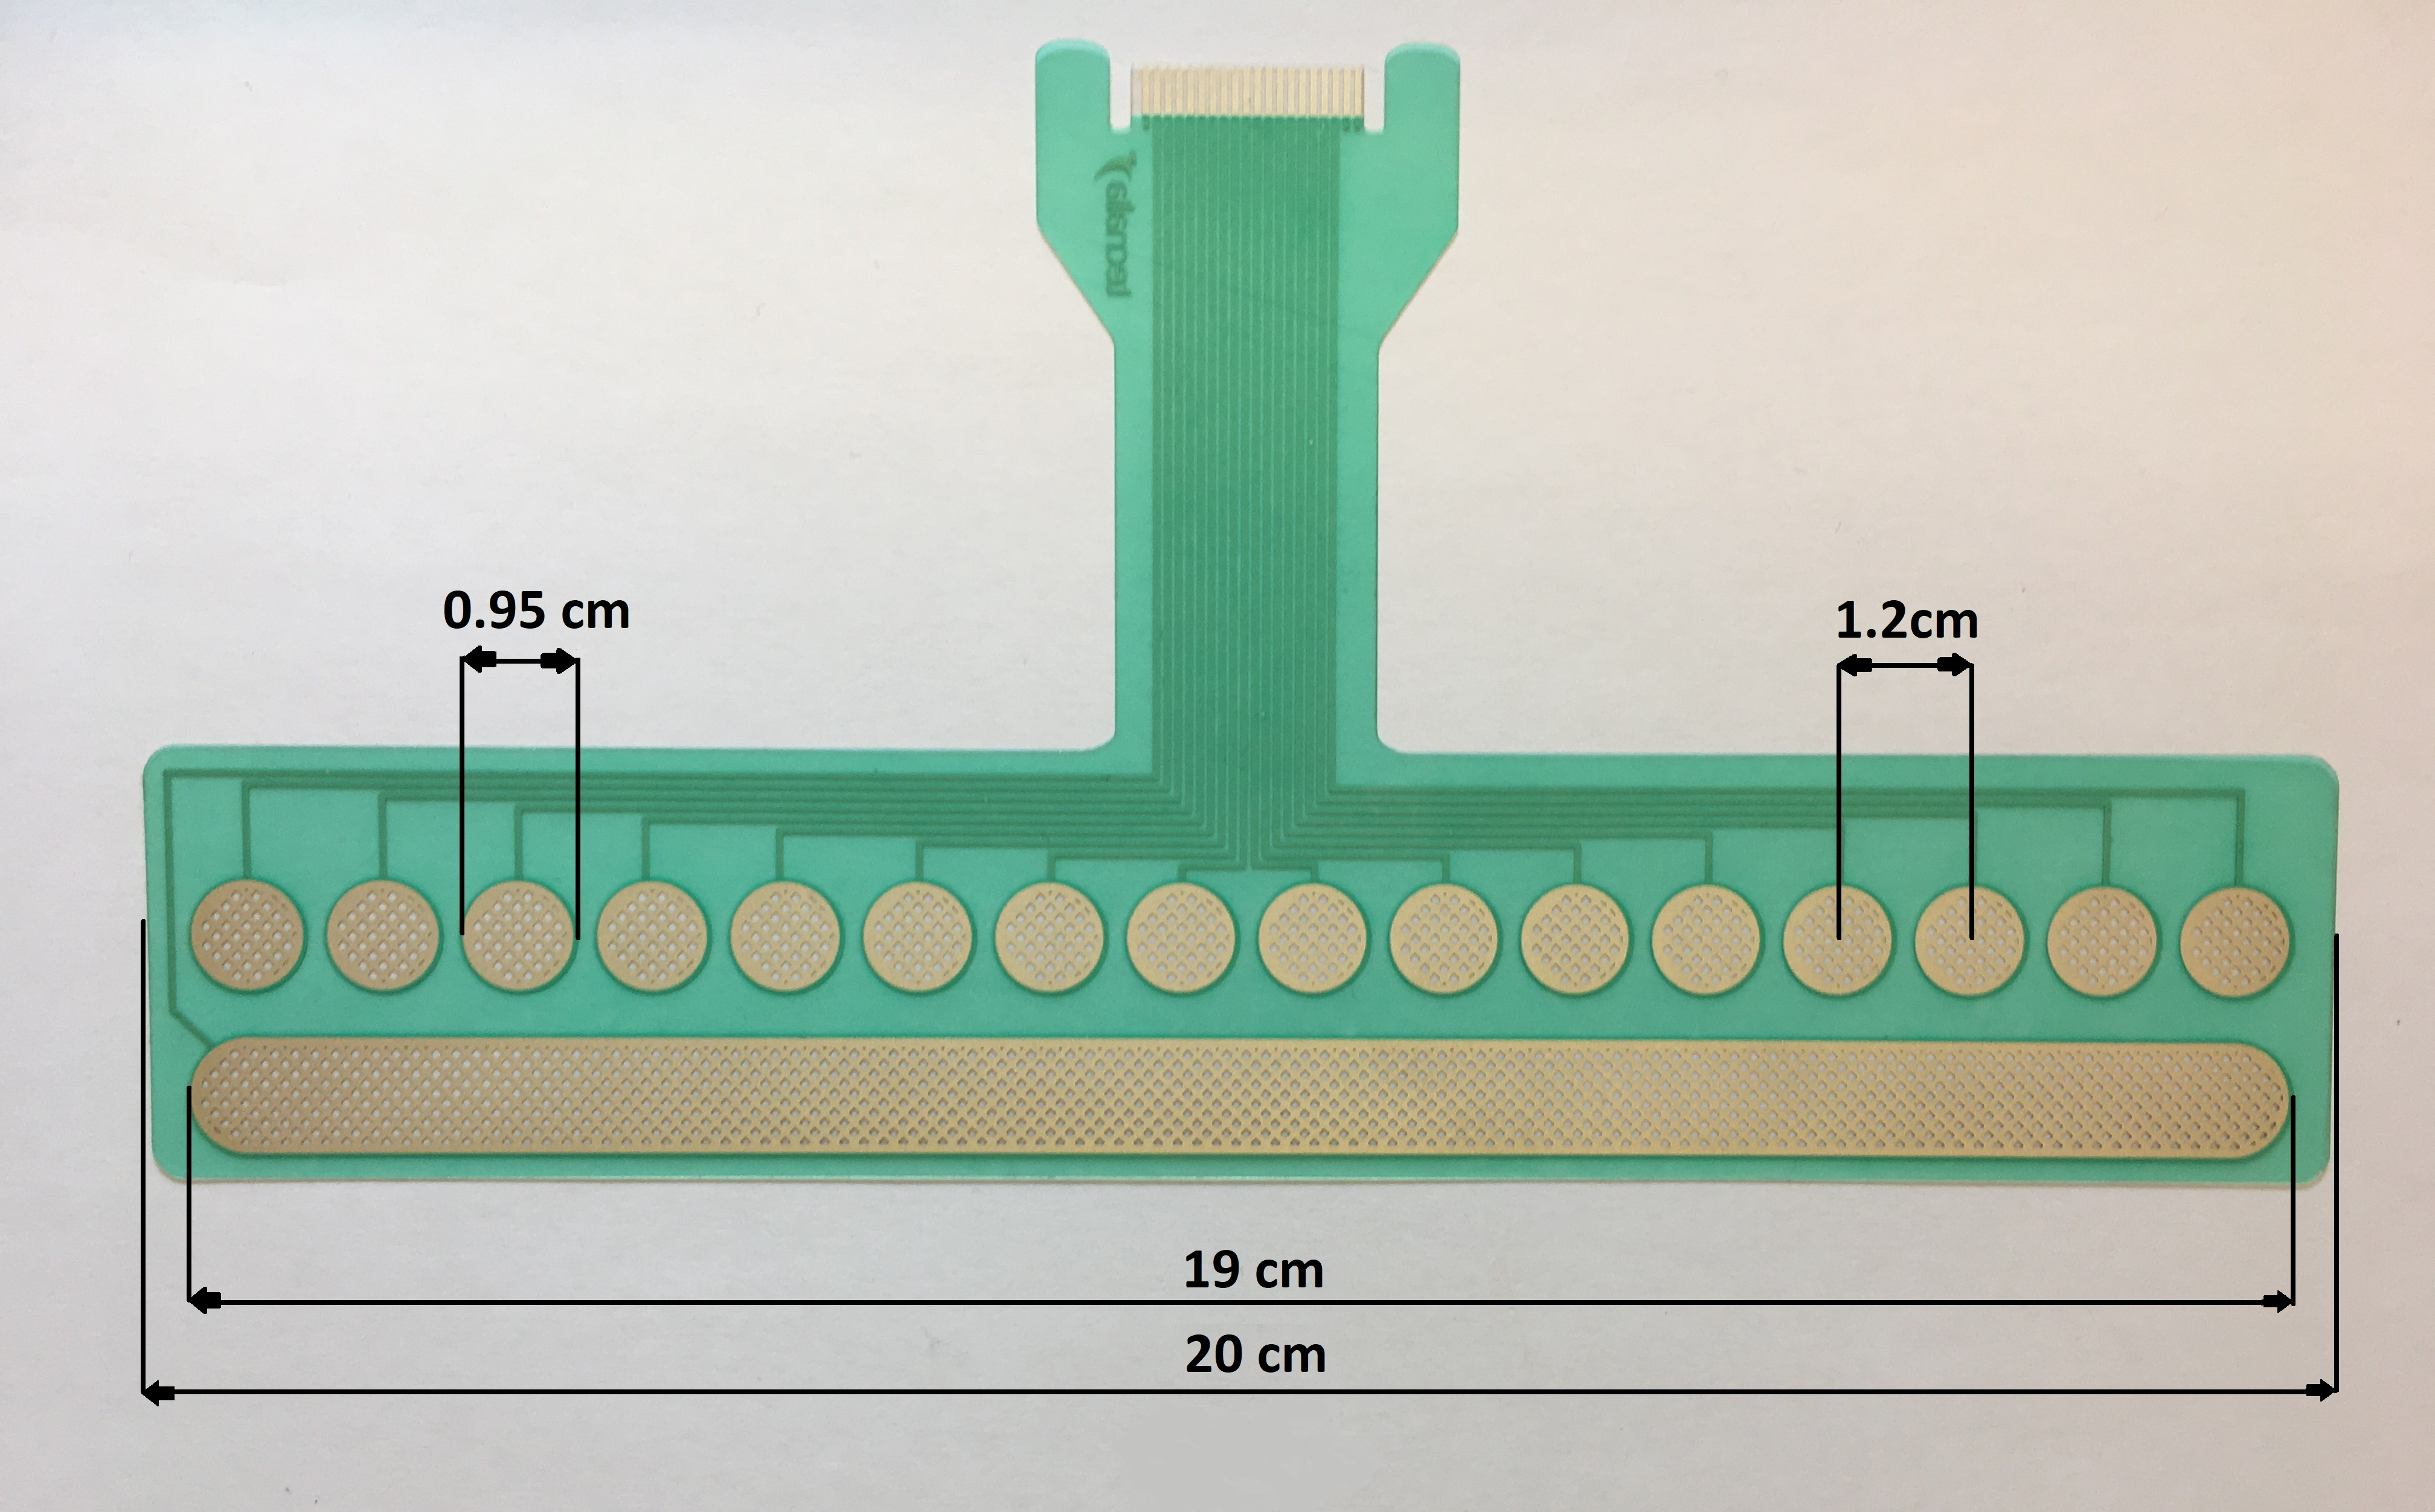
\includegraphics[width=1\textwidth]{figures/electrode}  
	\caption{Image of the 16 multi-pad electrode array used for stimulation. It consisted of 16 circular cathode pads, which each shared a common anode.}
	\label{fig:pa:electrode} 
\end{figure}
\begin{figure}[h]                 
	\includegraphics[width=1\textwidth]{figures/max}  
	\caption{The MaxSense stimulation device used for independently controlling the activation of each pad in the attached electrode array.}
	\label{fig:pa:max} 
\end{figure}   
The array electrode consisted of a single anode pad and 16 circular cathode pads. The pads comprised of conductive Ag/AgCl traces imprinted in a 150 $\mu$m thick polyester layer. All pads were covered with conductive hydrogel (AG702, Axelgaard, Denmark) to enhance skin-electrode contact.  A multichannel stimulation feedback device (MaxSens, Tecnalia, Spain), seen in figure \ref{fig:pa:max}, generating biphasic pulses was connected to a standard desktop PC for individual control of pad activation. The pulse width and amplitude could be modulated independently for each pad whereas the frequency was controlled globally. The pulse width could be modulated within a 50 - 1000 $\mu $s range with 10 $\mu $s steps, frequency ranges from 1 - 400 Hz with 1 Hz steps and current amplitude ranges from 50 - 10000 $\mu $A with 0.1 $\mu $A steps. The array electrode was placed circumferentially around the non-dominant arm to avoid interference with the EMG electrodes, which were fitted on the dominant arm. In a clinical application both interfaces should be placed on the same arm (residual limb). The stimulation electrodes were fitted such that the end pads had a maximum gap of 3 cm centrally on the volar side, when using a pronated arm as reference position. Hence, how distal the electrode array was placed towards the wrist depended on the diameter of the subject's forearm. The following sections will present the two developed feedback configurations. 


\subsubsection{Spatial configuration}

The motivation behind the spatial configuration was to communicate wrist rotation by spatially rotating dorsally placed active electrode pads and to communicate hand aperture by changing activation between volarly placed pads. 
This feedback design was chosen in order to intuitively mimic the directions of the motions in the included DoF's. An illustration of the spatial configuration can be seen in figure \ref{fig:pa:spatial}. The pads were divided into two groups each responsible for conveying information about a single DoF. The dorsally placed pads were allocated for wrist rotation and the volarly placed for hand aperture. The pads were furthermore paired such that each pair would represent one of four intervals of the feedback variable. For wrist rotation the pads were connected in side by side pairs. For right-handed subjects the activation of pad pairs would rotate laterally when increasing rotational states during supination and rotate medially during pronation. For the hand aperture DoF the pairs consisted of oppositely located pads on the medial and lateral sides. When increasing aperture states the active pairs would move volarly and the distance between active pads would become shorter. When both feedback variables were active, the pads pairs corresponding to the level of the hand aperture and rotational angle would be activated. Thus, a maximum of four pads could be active simultaneously. The reason for grouping adjacently placed pads to convey information about the rotational DoF was to improve sensation perception by stimulating a larger skin area, as shown in Dosen et al. \cite{Dosen2015}. 
\begin{figure}[h]                 
	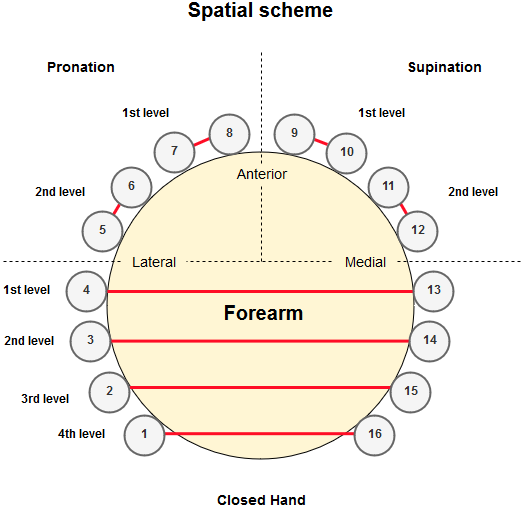
\includegraphics[width=.9\textwidth]{figures/El_array_spatial}  
	\caption{Transverse view of the developed spatial scheme fitted on the left arm of a subject. The levels written next to the pads pairs corresponded to the level of the position state; the higher the level, the higher the position state of the given movement was. When fitted on the right arm medial and lateral sides were reversed.}
	\label{fig:pa:spatial} 
\end{figure}   

\subsubsection{Amplitude configuration}
The incentive behind the amplitude configuration was to convey information by increasing the amplitude as the feedback variable increased. The feedback was provided in electrode pad groups of four.
The areas of active pads allocated for the various motions was similar to the spatial configuration to intuitively resemble the prosthesis motions. An illustration of the amplitude configuration can be seen in figure \ref{fig:pa:amplitude}. 
 \begin{figure}[h]                 
	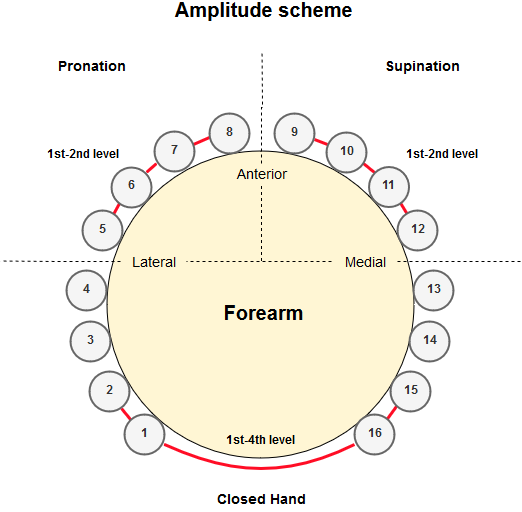
\includegraphics[width=.9\textwidth]{figures/El_array_amplitude}  
	\caption{Transverse view of the developed amplitude scheme fitted on the left arm of a subject. Different groups of four electrode pads were active during supination, pronation and hand aperture, respectively. The amplitude of the active pads would increase with the increase of the position state; the higher the position state level the higher the current amplitude of the given pads. When fitted on the right arm medial and lateral sides were reversed.}
	\label{fig:pa:amplitude} 
\end{figure}

The eight most dorsally placed pads were used for wrist rotation and the four most volarly placed pads for hand aperture. The eight pads used during wrist rotation were split such that the four most laterally placed were used during supination and four most medially placed were used during pronation for right-handed subjects. The pad activation was reversed for left-handed subjects. As the position state of a given movement would increase the current amplitude in the pads corresponding to that movement would increase. When in combined DoF position states, the pads corresponding to the level of the position state of each DoF would be active in the relative amplitude level. Thus, a maximum of eight pads could be active concurrently. The choice of grouping four electrode pads was decided upon to exploit the highest number of pads in the electrode array, while maintaining a symmetric distribution of possible active pads. Similarly to the spatial configuration this design was chosen to improve sensation perception \cite{Dosen2015}.




\textit{A. Experimental Protocol}

To investigate the usability of the developed feedback schemes in combination with control an experiment was conducted which evaluated the usefulness of the feedback schemes when eliminating visual dependency. For this purpose 14 able-bodied subjects (12 male and 2 female - 13 right-handed and 1 left-handed with a mean age of $26.1 \pm 2.4$ ) were recruited. Included subjects signed an informed consent form and meet inclusion criteria stated in the experimental protocol, which was ethically approved by the ethical committee of Region Nordjylland, Denmark (approval number N-20150075). Each subject was introduced, trained and finally evaluated in understanding both the spatially based scheme and the amplitude based scheme. However, the order of which feedback scheme the subject would be trained/tested in was randomized. \Figref{fig:std_pap} illustrates the chronological flow of stages in the experiment, where the first block focused on developing a subject specific prosthetic control system and the second block focused on training and evaluating the use of the sensory feedback schemes. 

\begin{figure}[H]                 
	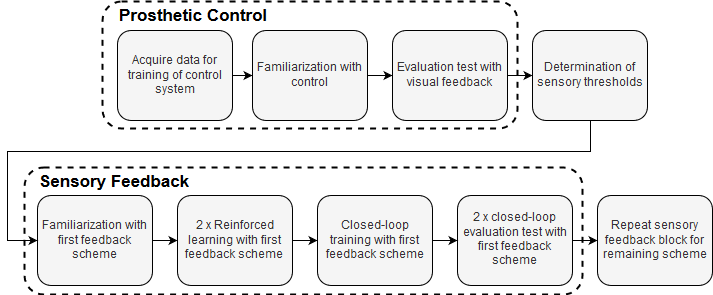
\includegraphics[width=.47\textwidth]{figures/std_paper}
	\caption{Pipeline showing the stages of the experiment. The stages in the first block focused on developing and evaluating a subject specific simulated prosthetic control system. Then electrotactile sensory thresholds were determined. The second block focused on training the understanding of the feedback schemes and evaluating their use in combination with prosthetic control.}
	\label{fig:std_pap} 
\end{figure}

During the first block, EMG data was initially acquired and used to train a control system, which was used for a simulate prosthetic control. Subsequently, was a stage where the subject was made familiar with the control system. Finally, the achieved prosthetic control was evaluated through a target reaching test. Afterwards, a series of subjects sensory thresholds were determined for use of conveying electrotactile feedback. The subject then began the stages of familiarizing and training with a feedback scheme followed by re-familiarization of control in combination with feedback. Finally, a evaluation test of using the sensory feedback in combination for control was made. The entire sensory feedback block was then repeated using the remaining feedback scheme. 





\subsection{Virtual Closed-Loop Prosthesis}
 \begin{figure*}[h]
		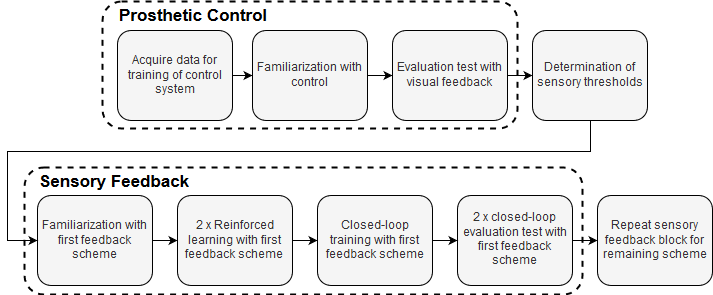
\includegraphics[width=.85\textwidth]{figures/std_paper}
	\caption{Pipeline showing the stages of the experiment. The stages in the first block focused on developing a prosthetic control system, and evaluating the subjects' ability to control the prosthesis. Then electrotactile sensory thresholds were determined. The second block focused on training the understanding of the feedback schemes and evaluating their use in combination with prosthetic control. The sensory feedback block was repeated for the remaining feedback scheme.}
	\label{fig:pa:std_pap} 
\end{figure*}
Investigating the usability of the two sensory configurations in a closed-loop scenario required these to be interfaced with a prosthetic device, which accommodated the actuation of rotational and hand aperture DoF's. However, using an actual prosthesis might result in auditory feedback being provided to the subject through prosthetic actuation sounds, eliminating the interest of solely exploring the impact of tactile feedback. Hence, it was chosen to simulate a velocity-based virtual prosthesis which enabled evaluation of the developed feedback schemes. In figure \ref{fig:pa:gridmap} is a depiction of a grid system, where the axes corresponded to the rotation angles and hand aperture. The grid squares represented the discrete intervals that were communicated through the feedback, where the cursor was the current angle and hand aperture. 
\begin{figure}[H]                 
	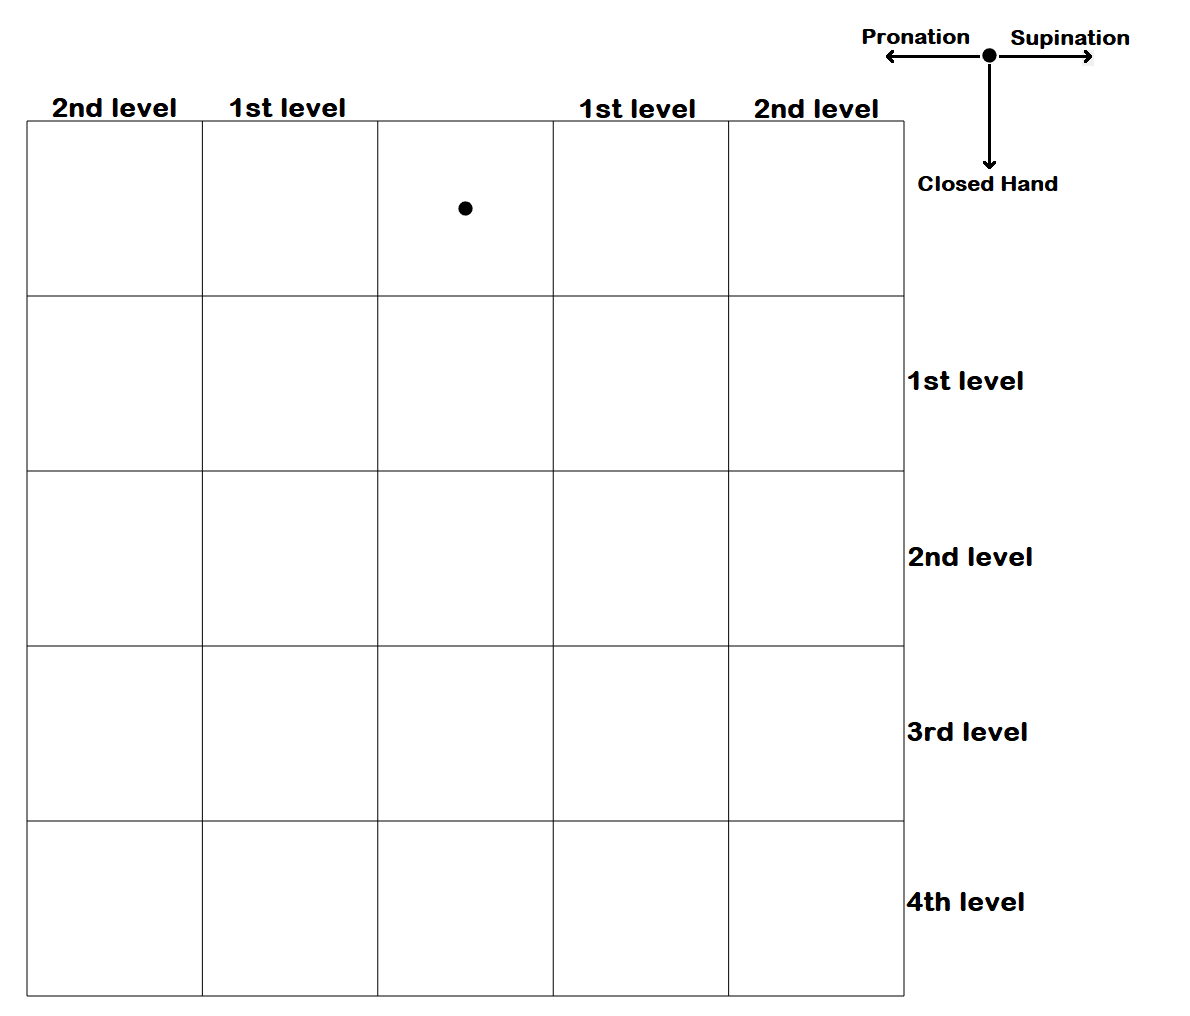
\includegraphics[width=1\textwidth]{figures/gridmap2}  
	\caption{Image of the grid map and cursor used in the experiment. Wrist supination moved the cursor to the right, pronation moved it to the left and closing the hand moved it downwards. For left-handed subjects, the rotational movements were reversed. Opening the hand moved the cursor upwards, and was used as a correction movement if needed.}
	\label{fig:pa:gridmap} 
\end{figure}

Performing supination would make the cursor move to the right and to the left when performing pronation. Performing closed hand would make the cursor move downwards and upwards when performing open hand, resembling the change in hand aperture. Performing rest (relaxing the arm) would make the cursor stand still. Furthermore, the contraction intensity was made proportional with the actuation speed, enabling the subject to have greater control of cursor movement speed. The control was sequential which only enabled the cursor to move in one DoF at a time. The control scheme thereby resembles what is typically used in commercial prostheses \cite{Atzori2015}. When the cursor entered a square a specific electrotactile stimulation would be provided corresponding to the stimulation pattern for each scheme. In the neutral position (location of cursor in figure \ref{fig:pa:gridmap}), no tactile feedback was provided.     



\section{Data Acquisition}

In order for a subject to be able to control the virtual prosthesis online, the prosthetic control system needed to be trained with previously acquired EMG signals. For EMG data acquisition the Myo Armband (MYB) from Thalmic labs was used, which contained eight dry stainless steel electrode pairs embedded on the inside of the armband. Furthermore, it could communicate wirelessly to external devices via a Bluetooth 4.0 unit, making it a highly practical recording device with minimum preparation time needed. However, it had a fixed sample rate of 200 Hz with the exclusive analogue filter being a 50 Hz notch filter, thus, making the EMG signals prone to aliasing. A study by Mendez et al. \cite{Mendez2017} showed, however, a similar mean classification accuracy of nine hand gestures in a LDA classifier, when comparing data acquired with electrodes that covered the entire EMG spectrum and MYB acquired data. This justified the use of the MYB and only a 10 Hz cut-off second order Butterworth high-pass filter was implemented digitally to remove low frequency artefacts. \\
To account for the delay until steady state motions was reached, it was desired to train the prosthetic control system with both transient and steady state EMG data from each movement \cite{Boschmann2013}. To archive this, the subjects was to follow a trapezoidal trajectory, where they controlled a cursor that moved horizontally with time in windows of 200 ms and vertically with EMG intensity. The recording was 11 seconds, where the trajectory had an incline/decline of two seconds and a plateau of five seconds, representing transient and steady state, respectively. The trajectory and cursor position was scaled relative to an initially recorded prolonged maximum voluntary contraction (pMVC) of 15 seconds, which was set to 1. Data was acquired from three recordings per movement, where the plateau was 40 $\percent$, 50 $\percent$ and 70 $\percent$ of the pMVC's, respectively. A last recording of 15 seconds rest was also performed.

\subsection{Feature extraction}
Features were extracted from the acquired EMG signals to expand the amount of information used to train the classifier in the prosthetic control system. Due to the risk of the EMG signals being aliased, features representing frequency content might lose fidelity. In a study by Donovan et al. \cite{Donovan2017}, the classification accuracy of space-domain features exploiting the relationship between EMG signals from neighbouring electrode pairs in the MYB were compared with the commonly used Hudgins features in a LDA classifier. Here, the use of space-domain features yielded a 5 $\percent$ higher accuracy than the Hudgins features with EMG data acquired from the MYB. It was therefore chosen to use the five non-redundant features derived by Donovan et al., along with the Hudgins feature Waveform Length to represent frequency content indirectly \cite{Hudgins1993}, resulting in a total of six features. Both offline and online features were extracted in windows of 200 ms with a 50 $\percent$ overlap to obtain quick update time, while preserving robust classification accuracy \cite{Menon2017}. 


\section{Prosthetic control system}
The extracted features were used to train a sequential proportional control system. For sequential control a LDA classifier was used and for proportional control multiple linear regression models were used. The following section will address the fitting of the control system. 

\subsection{Classification model}
A feature set was calculated for each of the eight electrode pairs and subsequently concatenated resulting in a 48-dimensional feature matrix that was provided to the classifier. It was chosen to implement a LDA classifier due to it being quick to train, while still yielding robust control \cite{Englehart2003}. The LDA classifier determined decision boundaries by maximizing the distance between centroids of the movement class feature values. Such decision boundaries were defined as a linear combination of feature values, where the output was posterior probabilities for each movement class. The decision rule was that the movement class with the highest probability would decide the determined motor function. The classifier was trained in distinguishing between five classes: wrist supination, wrist pronation, closed hand, opened hand and rest.  

\subsection{Proportional control}
The proportional control model provided the control system with an actuation velocity proportional to the contraction intensity in a direction based on which movement class that was decided on by the classifier. This was archived by training four multiple linear regression models: one for each active movement class. The mean absolute value (MAV) was calculated in windows for all electrode pairs and provided to the regression model as independent values, where the MAV scaled relative to the pMVC was provided as dependent values. During online control, the output was limited to a maximum value of 1; corresponding to the intensity of the pMVC. The distance of 1 corresponded to 1 cm on the computer screen, thus, the maximum speed of the virtual prosthesis was 1 cm per window (100 ms). A full DoF would be completed from one extremity to another in two seconds, thus, archiving an actuation velocity similar to the commercially available Bebionic prosthesis \cite{Belter2013}. A second restriction implemented was that a movement had to be performed with >15 $\percent$ contraction intensity, for the virtual prosthesis to be actuated. This was included to get a more stable resting state. 

\subsection{Subject Control Training and Evaluation} \label{sec:pa:subjectcontrol}
The subjects were initially trained in controlling the virtual prosthesis via visual feedback. It was crucial for subjects to achieve robust control for the feedback configurations to be able to be evaluated in a closed-loop prosthetic control system. The subjects' control abilities were assessed empirically during trainings and quantitatively through a Fitts' Law inspired target reaching test. If a subject did not have a completion rate above 90 $\%$ and a mean time to reach a target at below 10 seconds the subject would be excluded. 

The subject control training was divided into two runs of three minutes with a different prosthesis representation in each training. In the first training, the prosthesis was represented as a black cursor as seen in figure \ref{fig:pa:gridmap}. The cursor position would move continuously with each control system output. In the second training, the cursor was invisible, and the prosthesis representation was instead the square containing the cursor being highlighted. This discretized prosthesis representation was implemented to equalize the visual and sensory feedback. This prosthesis representation was used in the remaining training/test runs with visual feedback. During both training phases the subjects were instructed in practicing the ability to move the cursor in a desired direction and to transition from movement to rest. 

During the target reaching test, the subjects had to reach targets (highlighted grid squares) visualized in a randomized order. The subjects had to match the discretized virtual prosthesis with the target and dwell in that position for 1.5 seconds for it to be deemed reached. The subjects had 30 seconds to reach a target. If either a target was reached or the time limit was reached, the virtual prosthesis would reset in neutral position. The test was finished when all grid squares had been highlighted, making a total of 24 targets. 


\subsection{Determination of Electrotactile Sensory Thresholds}


Providing meaningful sensory feedback required determination of four distinguishable subject specific electrotactile thresholds. Threshold were made solely amplitude dependent by keeping pulse width and frequency constant at 500 $\mu s$ and 50 $Hz$, respectively. 1st level thresholds, termed perception thresholds, were determined for each pad by starting the amplitude at 0 $\mu A$ and then increasing in steps of 100 $\mu A$ per second. The subject was instructed to report when stimulation could be perceived confidently. Subsequently, the intensities were readjusted by comparing the sensation in each pad to the neighboring to achieve homogeneous sensations across all pads. \\
4th level thresholds, termed tolerance threshold, were set using the same approach, but initiating the amplitude value at the 1st level thresholds and increasing the amplitude in steps of 200 $\mu A$ per second. The thresholds were determined when the subject reported that the sensation was on the onset to getting unpleasant, the stimulation was becoming functional or a maximum of 10,000 $\mu A$ was reached. Intensities were again readjusted to achieve homogeneous sensations. Throughout the process of determining threshold the subject was was faced away from the screen. Intermediate threshold levels 2 and 3 were calculated for the $i^{th}$ pad based the perception and tolerance threshold as following. 
\vspace{-0.2cm}
{\small 
\begin{equation}
2~lvl(i) = perception(i) + (\frac{1}{3} \cdot (tolerance(i) - perception(i)))
\end{equation}}
{\small
\begin{equation}
3~lvl(i) = tolerance(i) - (\frac{1}{3} \cdot (tolerance(i) - perception(i)))
\end{equation}
}

\section{Sensory Feedback Training}

Following the subject training of prosthetic control, the subject was trained in understanding a sensory feedback scheme. The sensory feedback training was divided into two phases: familiarization and reinforced learning. \\
The familiarization phase provided the subjects with a short and controlled introduction to the scheme. The cursor was moved by the investigator from the neutral position to a designated state incorporating the transition from one square to the next, thus, presenting the subject with the coherence between states and stimulation patterns for a designated state. States in the top and bottom row and the middle column were presented actively, while the remaining 12 states were presented indirectly as transition states when moving to combinational states of 4th level closed hand and either 1st or 2nd level of wrist pronation and supination by first moving in the rotational DoF. Time spend in designated states was approximately four seconds and time spend in transition states was approximately two seconds. Recognition of single DoF states was assessed to be most crucial for comprehension, hence, these were favored in the familiarization phase. \\
For the reinforced learning phase the subject was asked to face away from the screen. The cursor was directed to a designated state and the subject then had to report what the current state was based solely on the sensory feedback. If the subject answered correctly, the cursor was reset to the neutral position and the cursor was moved to a new target. If the subject answered incorrectly, the correct state would be communicated for the subject to learn from, before continuing. Each state would be presented once and be moved to by taking the optimal path (move the cursor fully in one DoF before the other). However, which DoF the cursor would move in first was varied. Hence, the subject could utilize the transitions made when guessing the current state. The order of the designated states was pretermined by the investigators. Time spend in transition states was approximately two seconds. When all 24 states had been trained, the subject was given a short break before repeating the reinforced learning. However, the order and paths were changed for the second run.



\section{Closed-Loop System Evaluation}

Having completed the training of a feedback scheme its usability was evaluated through a evaluation test. \\
Before undergoing the test the subject was given a three minute familiarization period to get reacquainted with control familiarize with having to control the cursor while also focusing on perceiving the provided stimulation. \\
The evaluation test was similar to the evaluation test presented in \secref{sec:pa:subjectcontrol}. However, the cursor was not visualized, thus, the subject solely relied on sensory feedback, when moving to a targeted state. The evaluation test was performed two times consecutively.

\subsection{Statistical Analyses}
The metrics extracted from the evaluation tests were number of reached targets, time spend per target and path efficiency. Paired comparisons were made between results from evaluation tests. Due to the samples population not being normal-distributed following one-sample Kolmogorov-Smirnoff tests, comparisons were made using non-parametric statistics. Wilcoxon signed rank test was applied as comparisons was made on related samples obtained from a two block study design. A significance level of p < 0.05 was used.



\section{Results}


\subsection{Prosthesis Trajectories}

Figure \ref{fig:pa:trajec} illustrates two example prosthesis trajectories from the amplitude feedback evaluation test with combined DoF states as targets: one ideal trajectory (top figure) and one feedback assisted path correction (bottom figure). The ideal trajectory indicates a total comprehension of the feedback, where no overshoots or detours were performed. The feedback assisted path correction is an example of a subject overshooting the closed hand direction before performing supination. However, this was compensated for as the subject moved directly in a lower level closed hand state after reaching the correct rotational state. This illustrated the subject's ability to utilize the feedback when correcting for an overshoot. 

\begin{figure}[h]                 
	\includegraphics[width=.7\textwidth]{figures/trajectories}
	\caption{Examples of two prosthesis trajectories when reaching a combined DoF target in the amplitude evaluation test. The top figure shows an ideal trajectory and the bottom figure illustrates a feedback assisted path correction. The blue line is the prosthesis trajectory, the center of the green circle is the end position and the red square is the targeted state.}
	\label{fig:pa:trajec} 
\end{figure}

\subsection{Evaluation Metrics}
The evaluation metrics from first to second evaluation test in each feedback scheme did not yield significant difference (p > 0.05). Therefore, it was chosen to view these evaluation tests as one, by calculating the mean between the first and second evaluation test in both blocks, resulting in a single test result for the spatial feedback and a test single result for the amplitude feedback. 

Figure \ref{fig:pa:boxplot_results} shows box plots of the extracted metrics for the visual, spatial and amplitude feedback evaluation tests. Worth noting was that visual feedback still outperformed solely relying on electrotactile feedback both when spatially or amplitude modulated for the completion rate and time to reach a target metrics. When comparing the spatial and amplitude feedback tests, using amplitude feedback yielded a slightly higher completion rate (p = 0.044). This quantitative result was also supported by the subjective opinion of the subjects as 64 \% of the subjects favored the amplitude feedback. However, all subjects struggled in choosing a favored feedback scheme as they found both intuitive to understand. 


\subsection{Target State Hit Distribution}

When observing the completion rate of the specific targets in figure \ref{fig:pa:hit_dist}, it can be derived that targets generally had a higher hit rate when using amplitude feedback compared to spatial (mean completion rate with spatial feedback was 87 \% $\pm$ 11 \% and amplitude was 93 \% $\pm$ 6 \%). However, common for both feedback scheme was that the centered targets were more troublesome to reach (mean completion rate for centered targets was 76 \% $\pm$ 10 \%  with spatial feedback and 88 \%  $\pm$ 4 \% with amplitude feedback; mean completion rate for peripheral targets was 93 \% $\pm$ 6 \% with spatial feedback and 97 \% $\pm$ 3 \% with amplitude feedback). A possible reason for this finding is that the subjects had to achieve complete rest to dwell inside these targets. In the peripheral targets, the subjects did not necessarily need to achieve complete rest, as they could continue performing a movement and still be on the boundary of the target. 

Furthermore, combined DoF targets generally had a lower completion rate for the spatial feedback scheme (mean completion rate for single DoF targets was 90 \% $\pm$ 12 \% with spatial feedback and 93 \% $\pm$ 6 \% with amplitude feedback; mean completion rate for combined DoF targets was 85 \% $\pm$ 11 \% with spatial feedback and 93 \% $\pm$ 6 \% with amplitude feedback). This could indicate that the sensory feedback regarding combined prosthetic states in the spatial feedback scheme was slightly harder to interpret than in the amplitude feedback scheme. 


\begin{figure*}[h]                 
	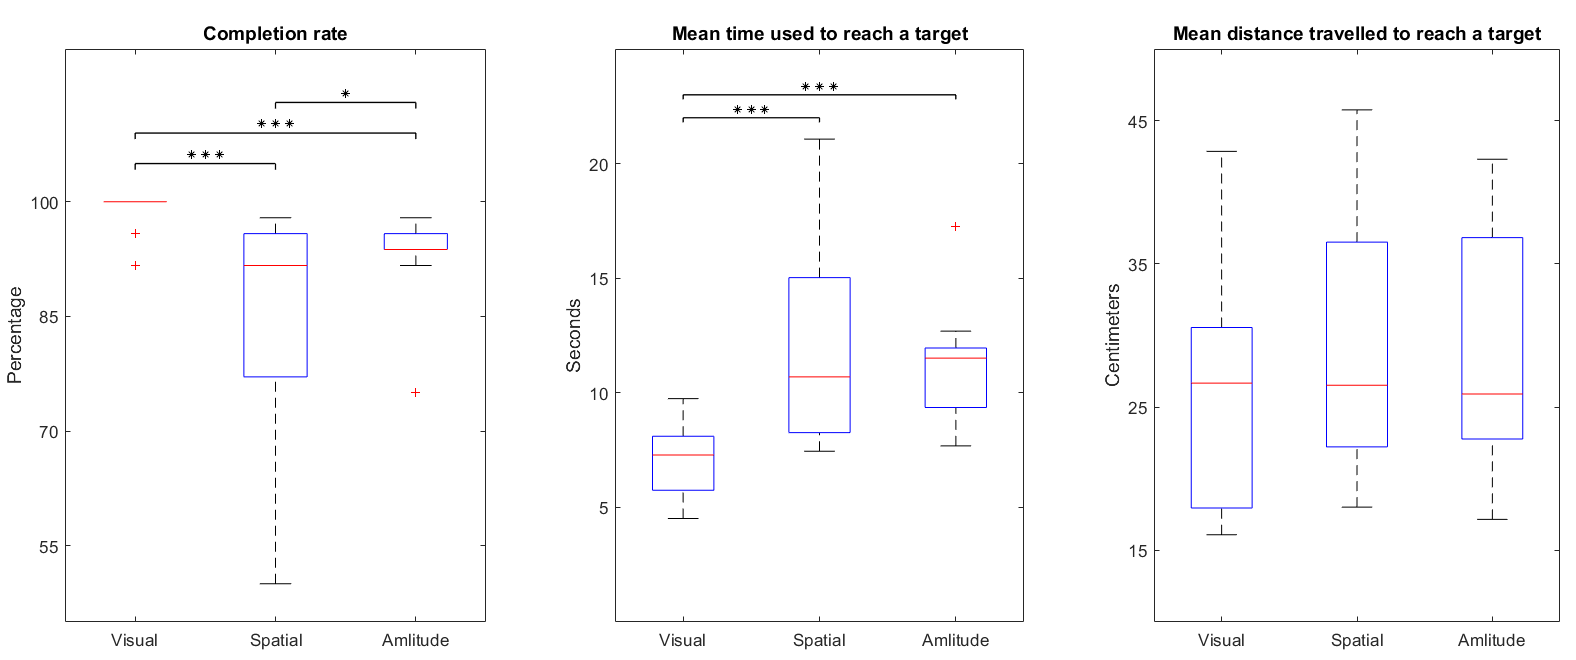
\includegraphics[width=1\textwidth]{figures/boxplot_results}
	\caption{Box plots of the metrics extracted from the visual, spatial and amplitude feedback evaluation tests. The two evaluation tests in the spatial and amplitude feedback block, respectively, were combined by calculating the mean between the two tests. One asterisk indicates p-value < 0.05 and three asterisks indicates p-value < 0.001.}
	\label{fig:pa:boxplot_results} 
\end{figure*}

\begin{figure}[H]                 
	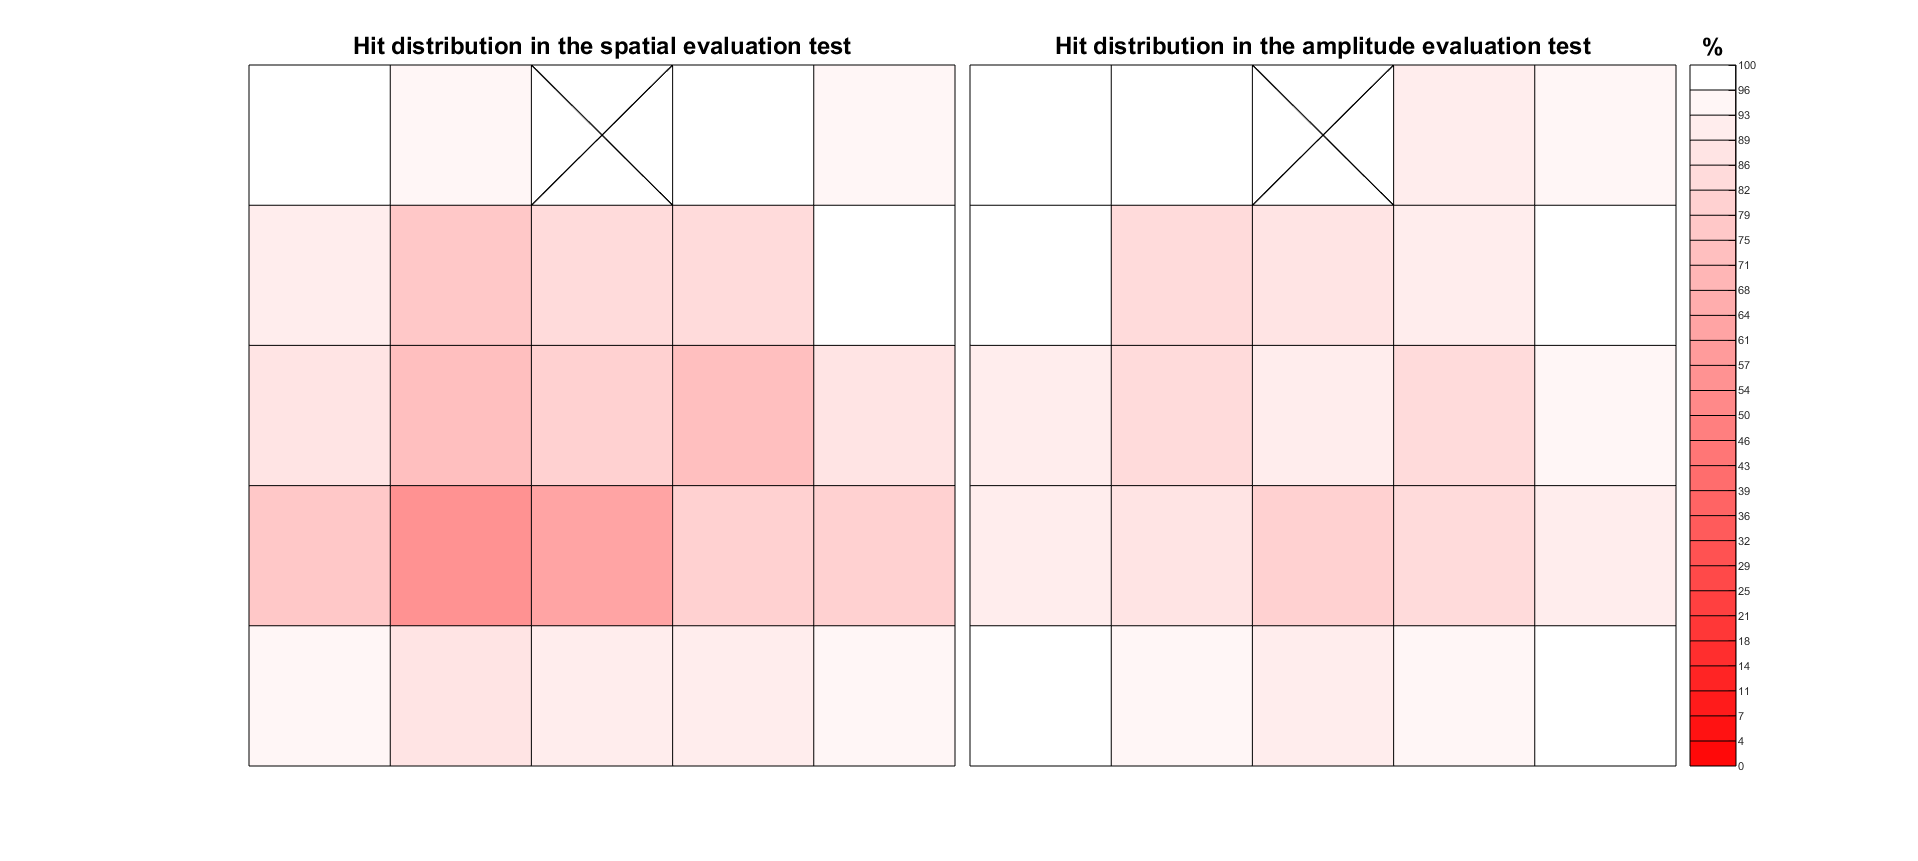
\includegraphics[width=.7\textwidth]{figures/hit_dist}
	\caption{Hit rate for each target in the spatial and amplitude evaluation test, respectively. The more transparent a target is, the higher the hit rate was. 100 $\%$ accounts for a total of 28 hits for each test.}
	\label{fig:pa:hit_dist} 
\end{figure}




\section{Discussion}

Two intuitive electrotactile feedback schemes were developed for a two DoF velocity-based virtual prosthesis: one spatially modulated and one amplitude modulated. The schemes were integrated in an easy implementable 16 pad electrode array and tested in combination with sequential proportional myoelectric control. Unique sensory feedback was provided for four levels of prosthetic states in single DoF's and for 16 prosthetic states representing combined DoF's. The objective was to investigate the usability of the developed feedback schemes when removing visual dependency.

From the metrics extracted describing the subjects' performance in the evaluation test, only completion rate indicated a slight  dominance in favor of the amplitude scheme compared to the spatial scheme (p-value = 0.044). However, with a mean completion rate of 93 \% $\pm$ 6 \% and 87 \% $\pm$ 11 \%, respectively, both feedback schemes can be deemed intuitive to utilize in combination with myoelectric control when removing visual dependency. Considering that these completion rates were obtained from a minimal training protocol (training time per scheme < 30 minutes), a completion rate similar to visual feedback (99 $\% \pm 2\%$) might be achieved if more training blocks were included.
Compared to the results of Strbac et al. \cite{Strbac2016} the results of recognizing more complex four DoF stimulation patterns which achieved a success rate of 99 $\% \pm 3\%$ for able-bodied subjects, the usability of the derived schemes seems lower. However, Strbac et al. did not test the usability of their feedback schemes in combination with control. Furthermore, recognizability was only investigated for each DoF independently and not in combinations as in this study. We speculate, that eliminating these variables, similar results would be achieved when subjects were given adequate training time.       

In the reinforced learning, the mean success rate for the spatial scheme was 73 \%  $\pm$ 17 \% and 78 \%  $\pm$ 16 \% for the amplitude scheme. This was a notably lower success rate than obtained from the closed-loop evaluation tests. This could indicate that when put into the intended application, a higher understanding of the feedback can be accomplished. If the training block had the same duration, but was solely closed-loop-based, an even higher success rate might have been achieved in the evaluation tests. 

\subsection{Sensory Thresholds}
Some subjects reported that it was difficult to separate levels in both DoF's in the spatial scheme, due to a notable difference in sensation intensity between levels. A different approach in the determination of sensory threshold levels might have removed this confusion in the spatial feedback. The amplitude levels were determined by setting the threshold level for the electrode pads in a consecutive order. This might have caused a slight adaptation in the sensory perception of the subjects, which distorted the sensation intensity when applied in the sensory feedback training and the evaluation tests. By interleaving the order of designated electrode pads, or by making the determination of threshold levels more scheme related (setting threshold levels simultaneously for pads connected in the schemes), could have made the sensation intensities more homogeneous across all pads. A weak functional electrical stimulation due to summation of active stimulation pads was observed in few subjects during the amplitude sensory feedback training, and might also have been avoided by relating the determination of threshold levels to the schemes. 

%Subject maxing out the amplitude during determination of thresholds.
\subsection{Future Works}
As mentioned, even with a minimal training, the results indicated a clear intuitiveness in understanding both feedback schemes. In that context, it would of great interest to investigate the performance of the feedback scheme concepts in a less discretized environment. With the electrode array used in this study, especially the amplitude scheme has a huge potential, as only the device restrictions and subjects' sensory discrimination abilities are a limit.
In the evaluation tests, only the active movement of the grasping DoF (closing the hand) was assessed, and the starting point was always resting state (no feedback received). In future studies, it could be investigated how the performance would be if the starting point was varied, e.g. by randomizing the starting point to resting state and highest level hand aperture, or by not resetting the prosthetic state when a new target state appeared. This would demand the subjects to more comprehensive understand the feedback, as they would not as rigidly be given reference states during the tests, and the test would be more transferable to practical prosthetic use.

Finally, as the schemes were easy comprehensible, an expansion of the scheme concepts to represent more DoF's would be a large step towards producing a prosthetic device concept with the potential of enhancing the users' prosthetic embodiment. Since electrotactile stimulation allows for modulation of frequency, another DoF could be included enhancing the complexity and amount of information which can be conveyed. For instance, proportional grasp force feedback was the most important feedback to restore according to \cite{Peerdeman2011}. This could be restored using frequency in a similar fashion as done in \cite{Dosen2016}, where grasp force was modulated via stimulation frequency. 
 
%Make comparison between amplitude and frequency modulated feedback. 





\section{Conclusion}


\appendix[Acknowledgement]
The authors would like to thank supervisors Strahinja Dosen and Jakob Lund Dideriksen for providing constructive feedback, and the School of Medicine and Health at Aalborg University for providing equipment and the facilities to complete this study. Additionally, the authors are very thankful for all the voluntary participants. 
%\clearpage
%\IEEEtriggeratref{16}  % Cuts the references so the equalizes in length in the two coloums (x) is the reference number where the cut should be made
\bibliography{bibliography}
\bibliographystyle{ieeetr}

\end{document}

